\documentclass[border=6pt]{standalone}
\usepackage{tikz}
\usepackage{pgfplots}
\pgfplotsset{compat=1.18}
\usetikzlibrary{arrows.meta,positioning,shapes.geometric,fit,backgrounds,calc,decorations.pathreplacing,patterns}
\usetikzlibrary{pgfplots.groupplots}
\tikzset{
  blk/.style={rectangle, rounded corners=2pt, draw=black!70, thick, fill=blue!6,
              minimum height=8mm, minimum width=20mm, align=center, font=\small},
  io/.style={rectangle, rounded corners=6pt, draw=black!70, thick, fill=green!8,
             minimum height=8mm, align=center, font=\small},
  proc/.style={rectangle, draw=black!70, thick, fill=orange!10, minimum height=8mm,
               align=center, font=\small},
  dec/.style={diamond, aspect=2, draw=black!70, thick, fill=yellow!15, align=center, font=\footnotesize},
  warnbox/.style={rectangle, rounded corners=2pt, draw=red!60!black, thick, fill=red!7,
                  minimum height=8mm, align=center, font=\small},
  oklbox/.style={rectangle, rounded corners=2pt, draw=green!45!black, thick, fill=green!8,
                 minimum height=8mm, align=center, font=\small},
  ar/.style={-{Latex[length=2mm]}, thick},
  arl/.style={-{Latex[length=2mm]}, thick, dashed, draw=black!55},
  lbl/.style={font=\footnotesize\itshape, text=black!60},
}
\definecolor{good}{RGB}{34,139,34}
\definecolor{bad}{RGB}{178,34,34}
\definecolor{warn}{RGB}{218,165,32}
\definecolor{pesblue}{RGB}{0,45,98}
\definecolor{complete}{RGB}{30,125,79}
\definecolor{partial}{RGB}{176,106,0}
\definecolor{blocked}{RGB}{166,43,43}
\begin{document}
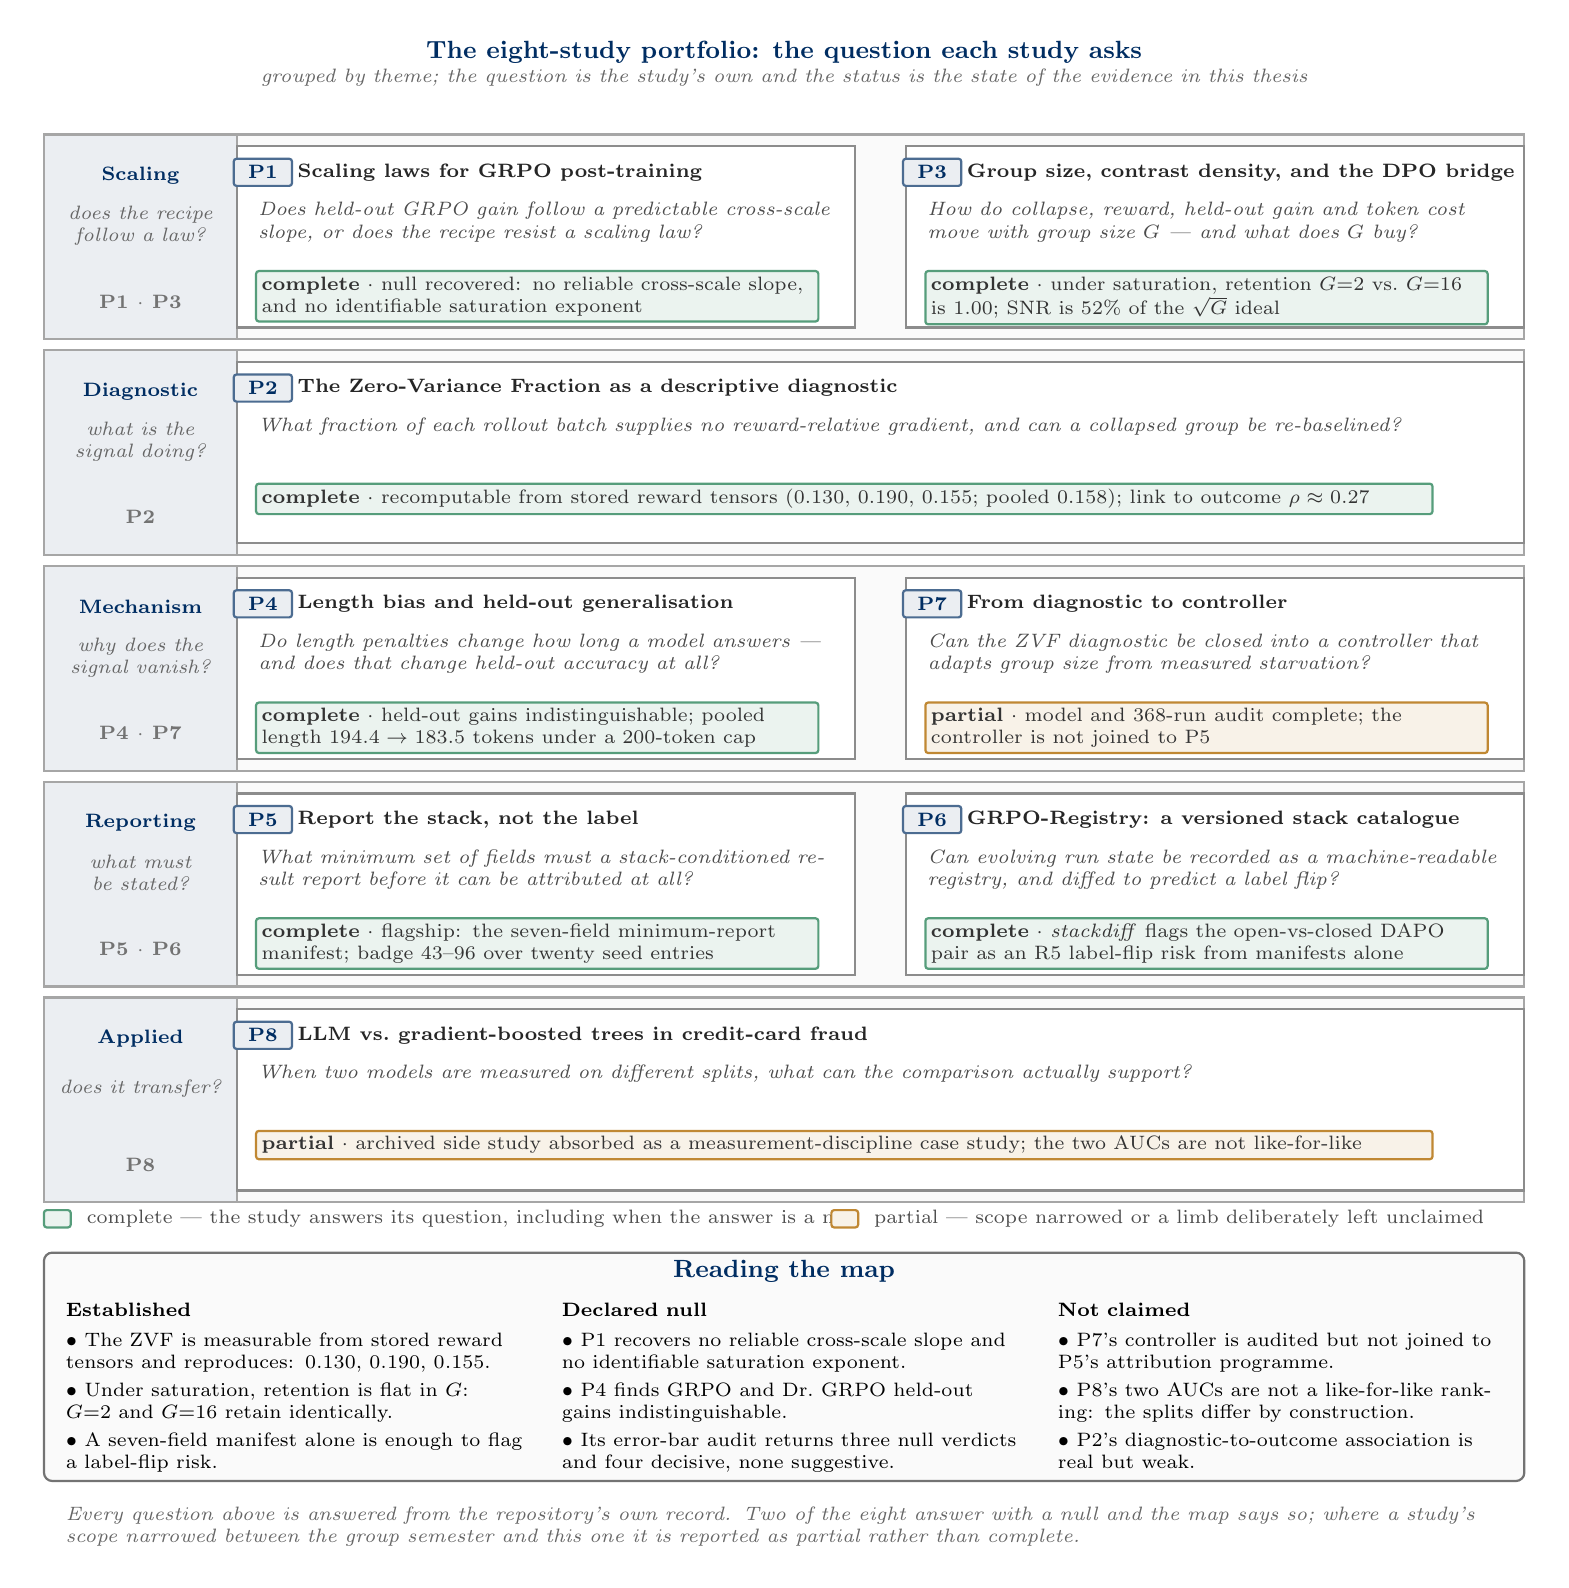
\begin{tikzpicture}[x=1cm,y=1cm,
  hdt/.style={font=\small\bfseries, text=pesblue, align=center, inner sep=1pt},
  hds/.style={font=\scriptsize\itshape, text=black!60, align=center, inner sep=1pt},
  thn/.style={font=\scriptsize\bfseries, text=pesblue, align=center, text width=2.20cm, inner sep=1pt},
  thg/.style={font=\scriptsize\itshape, text=black!60, align=center, text width=2.20cm, inner sep=1pt},
  thi/.style={font=\scriptsize\bfseries, text=black!55, align=center, inner sep=1pt},
  card/.style={draw=black!45, thick, fill=white},
  rqchip/.style={rectangle, rounded corners=1pt, draw=pesblue!70, thick, fill=pesblue!8,
                 font=\scriptsize\bfseries, text=pesblue, inner sep=2.5pt,
                 minimum width=0.74cm, align=center},
  rqt/.style={anchor=west, font=\scriptsize\bfseries, text=black!85, align=left, inner sep=1pt},
  rqqw/.style={anchor=north west, font=\scriptsize\itshape, text=black!70, align=left,
               inner sep=1pt, text width=15.60cm},
  rqqn/.style={anchor=north west, font=\scriptsize\itshape, text=black!70, align=left,
               inner sep=1pt, text width=7.35cm},
  stc/.style={rectangle, rounded corners=1pt, draw=complete!75, thick, fill=complete!9,
              font=\scriptsize, text=black!80, align=left, inner sep=2pt,
              anchor=north west, text width=7.00cm},
  stp/.style={rectangle, rounded corners=1pt, draw=partial!80, thick, fill=partial!9,
              font=\scriptsize, text=black!80, align=left, inner sep=2pt,
              anchor=north west, text width=7.00cm},
  stcw/.style={stc, text width=14.80cm},
  stpw/.style={stp, text width=14.80cm},
  pnote/.style={font=\scriptsize, align=left, inner sep=2pt, anchor=north west},
]
% invisible path: fixes the bounding box
\draw[opacity=0] (-9.60,5.25) rectangle (9.60,-14.20);

% ================= HEADER =================
\node[hdt] at (0,4.95) {The eight-study portfolio: the question each study asks};
\node[hds, text width=18.60cm] at (0,4.62)
  {grouped by theme; the question is the study's own and the status is the state of the
   evidence in this thesis};

% ================= BAND FRAMES =================
\foreach \bt in {3.90, 1.16, -1.58, -4.32, -7.06}{
  \fill[black!2] (-9.40,\bt) rectangle (9.40,{\bt-2.60});
  \fill[pesblue!8] (-9.40,\bt) rectangle (-6.95,{\bt-2.60});
  \draw[black!35, thick] (-9.40,\bt) rectangle (9.40,{\bt-2.60});
  \draw[black!35, thick] (-6.95,\bt) -- (-6.95,{\bt-2.60});
}

% ================= THEME STRIPS =================
% -- scaling --
\node[thn] at (-8.175, 3.38) {Scaling};
\node[thg] at (-8.175, 2.74) {does the recipe follow a law?};
\node[thi] at (-8.175, 1.78) {P1 $\cdot$ P3};
% -- diagnostic --
\node[thn] at (-8.175, 0.64) {Diagnostic};
\node[thg] at (-8.175, 0.00) {what is the signal doing?};
\node[thi] at (-8.175,-0.96) {P2};
% -- mechanism --
\node[thn] at (-8.175,-2.10) {Mechanism};
\node[thg] at (-8.175,-2.74) {why does the signal vanish?};
\node[thi] at (-8.175,-3.70) {P4 $\cdot$ P7};
% -- reporting / infrastructure --
\node[thn] at (-8.175,-4.84) {Reporting};
\node[thg] at (-8.175,-5.48) {what must be stated?};
\node[thi] at (-8.175,-6.44) {P5 $\cdot$ P6};
% -- applied --
\node[thn] at (-8.175,-7.58) {Applied};
\node[thg] at (-8.175,-8.22) {does it transfer?};
\node[thi] at (-8.175,-9.18) {P8};

% =======================================================================
% BAND 1 -- scaling: P1, P3
% =======================================================================
\draw[card] (-6.95,3.75) rectangle (0.90,1.45);
\node[rqchip] at (-6.62,3.42) {P1};
\node[rqt] at (-6.22,3.42) {Scaling laws for GRPO post-training};
\node[rqqn] at (-6.72,3.08)
  {Does held-out GRPO gain follow a predictable cross-scale slope, or does the recipe
   resist a scaling law?};
\node[stc] at (-6.72,2.18)
  {\textbf{complete} $\cdot$ null recovered: no reliable cross-scale slope, and no
   identifiable saturation exponent};

\draw[card] (1.55,3.75) rectangle (9.40,1.45);
\node[rqchip] at (1.88,3.42) {P3};
\node[rqt] at (2.28,3.42) {Group size, contrast density, and the DPO bridge};
\node[rqqn] at (1.78,3.08)
  {How do collapse, reward, held-out gain and token cost move with group size $G$ ---
   and what does $G$ buy?};
\node[stc] at (1.78,2.18)
  {\textbf{complete} $\cdot$ under saturation, retention $G{=}2$ vs.\ $G{=}16$ is $1.00$;
   SNR is $52\%$ of the $\sqrt{G}$ ideal};

% =======================================================================
% BAND 2 -- diagnostic: P2 (single study, full-width card)
% =======================================================================
\draw[card] (-6.95,1.01) rectangle (9.40,-1.29);
\node[rqchip] at (-6.62,0.68) {P2};
\node[rqt] at (-6.22,0.68) {The Zero-Variance Fraction as a descriptive diagnostic};
\node[rqqw] at (-6.72,0.34)
  {What fraction of each rollout batch supplies no reward-relative gradient, and can a
   collapsed group be re-baselined?};
\node[stcw] at (-6.72,-0.52)
  {\textbf{complete} $\cdot$ recomputable from stored reward tensors (0.130, 0.190, 0.155;
   pooled 0.158); link to outcome $\rho \approx 0.27$};

% =======================================================================
% BAND 3 -- mechanism: P4, P7
% =======================================================================
\draw[card] (-6.95,-1.73) rectangle (0.90,-4.03);
\node[rqchip] at (-6.62,-2.06) {P4};
\node[rqt] at (-6.22,-2.06) {Length bias and held-out generalisation};
\node[rqqn] at (-6.72,-2.40)
  {Do length penalties change how long a model answers --- and does that change held-out
   accuracy at all?};
\node[stc] at (-6.72,-3.30)
  {\textbf{complete} $\cdot$ held-out gains indistinguishable; pooled length
   $194.4 \rightarrow 183.5$ tokens under a $200$-token cap};

\draw[card] (1.55,-1.73) rectangle (9.40,-4.03);
\node[rqchip] at (1.88,-2.06) {P7};
\node[rqt] at (2.28,-2.06) {From diagnostic to controller};
\node[rqqn] at (1.78,-2.40)
  {Can the ZVF diagnostic be closed into a \mbox{controller} that adapts group size
   from measured starvation?};
\node[stp] at (1.78,-3.30)
  {\textbf{partial} $\cdot$ model and 368-run audit complete; the \mbox{controller}
   is not joined to P5};

% =======================================================================
% BAND 4 -- reporting / infrastructure: P5, P6
% =======================================================================
\draw[card] (-6.95,-4.47) rectangle (0.90,-6.77);
\node[rqchip] at (-6.62,-4.80) {P5};
\node[rqt] at (-6.22,-4.80) {Report the stack, not the label};
\node[rqqn] at (-6.72,-5.14)
  {What minimum set of fields must a stack-conditioned result report before it can be
   attributed at all?};
\node[stc] at (-6.72,-6.04)
  {\textbf{complete} $\cdot$ flagship: the seven-field minimum-report manifest; badge
   $43$--$96$ over twenty seed entries};

\draw[card] (1.55,-4.47) rectangle (9.40,-6.77);
\node[rqchip] at (1.88,-4.80) {P6};
\node[rqt] at (2.28,-4.80) {GRPO-Registry: a versioned stack catalogue};
\node[rqqn] at (1.78,-5.14)
  {Can evolving run state be recorded as a machine-readable registry, and diffed to
   predict a label flip?};
\node[stc] at (1.78,-6.04)
  {\textbf{complete} $\cdot$ \textit{stackdiff} flags the open-vs-closed DAPO pair as an
   R5 label-flip risk from manifests alone};

% =======================================================================
% BAND 5 -- applied: P8 (single study, full-width card)
% =======================================================================
\draw[card] (-6.95,-7.21) rectangle (9.40,-9.51);
\node[rqchip] at (-6.62,-7.54) {P8};
\node[rqt] at (-6.22,-7.54) {LLM vs.\ gradient-boosted trees in credit-card fraud};
\node[rqqw] at (-6.72,-7.88)
  {When two models are measured on different splits, what can the comparison actually
   support?};
\node[stpw] at (-6.72,-8.74)
  {\textbf{partial} $\cdot$ archived side study absorbed as a measurement-discipline case
   study; the two AUCs are not like-for-like};

% =======================================================================
% STATUS LEGEND
% =======================================================================
\filldraw[fill=complete!9, draw=complete!75, thick, rounded corners=1pt]
  (-9.40,-9.98) rectangle (-9.06,-9.76);
\node[anchor=west, font=\scriptsize, text=black!70] at (-8.98,-9.87)
  {complete --- the study answers its question, including when the answer is a null};
\filldraw[fill=partial!9, draw=partial!80, thick, rounded corners=1pt]
  (0.60,-9.98) rectangle (0.94,-9.76);
\node[anchor=west, font=\scriptsize, text=black!70] at (1.02,-9.87)
  {partial --- scope narrowed or a limb deliberately left unclaimed};

% =======================================================================
% READING THE MAP
% =======================================================================
\draw[draw=black!55, thick, rounded corners=3pt, fill=black!2]
  (-9.40,-10.30) rectangle (9.40,-13.20);
\node[hdt] at (0,-10.54) {Reading the map};

\node[pnote, text width=5.80cm] at (-9.20,-10.86)
  {\textbf{Established}\\[3pt]
   $\bullet$ The ZVF is measurable from stored reward tensors and reproduces:
   $0.130$, $0.190$, $0.155$.\\[2pt]
   $\bullet$ Under saturation, retention is flat in $G$: $G{=}2$ and $G{=}16$ retain
   identically.\\[2pt]
   $\bullet$ A seven-field manifest alone is enough to flag a label-flip risk.};

\node[pnote, text width=5.80cm] at (-2.90,-10.86)
  {\textbf{Declared null}\\[3pt]
   $\bullet$ P1 recovers no reliable cross-scale slope and no identifiable saturation
   exponent.\\[2pt]
   $\bullet$ P4 finds GRPO and Dr.\ GRPO held-out gains indistinguishable.\\[2pt]
   $\bullet$ Its error-bar audit returns three null verdicts and four decisive, none
   suggestive.};

\node[pnote, text width=5.80cm] at (3.40,-10.86)
  {\textbf{Not claimed}\\[3pt]
   $\bullet$ P7's controller is audited but not joined to P5's attribution
   programme.\\[2pt]
   $\bullet$ P8's two AUCs are not a like-for-like ranking: the splits differ by
   construction.\\[2pt]
   $\bullet$ P2's diagnostic-to-outcome association is real but weak.};

\node[font=\scriptsize\itshape, text=black!60, align=left, text width=18.60cm,
      anchor=north west, inner sep=2pt] at (-9.20,-13.45)
  {Every question above is answered from the repository's own record. Two of the eight
   answer with a null and the map says so; where a study's scope narrowed between the
   group semester and this one it is reported as partial rather than complete.};

\end{tikzpicture}
\end{document}
